\documentclass[conference]{IEEEtran}
\usepackage{enumerate}
\usepackage{graphics}
\usepackage{graphicx}
\usepackage{amsmath}
\usepackage{amssymb}
\usepackage{times}
\usepackage{bbm}
\usepackage[bb=boondox]{mathalfa}
\usepackage{multirow}
\usepackage{arydshln}
\usepackage{tikz}
\usepackage{bbold}
\usetikzlibrary{matrix}
\usepackage{subcaption}
\usepackage{url}

\begin{document}
\title{
Drive-by-Wire
\\[0.5cm]
\large{Studies on Mechatronics FS 2017}
}

\author{\IEEEauthorblockN{Noah Isaak}
\IEEEauthorblockA{student number: \\ 13-929-476}
\and

\IEEEauthorblockN{Richard von Moos}
\IEEEauthorblockA{student number: \\ 14-935-740}
}

\maketitle

%% Definitions by LF
\setlength\parindent{0pt}
\newcommand{\spn}[1]{\textsc{Span} \left\{ #1 \right\}}
\newcommand{\dimension}[1]{\textsc{dim} \left\{ #1 \right\}}
\newcommand{\real}[1]{\textsc{Re} \left( #1 \right)}
\newcommand{\imag}[1]{\textsc{Im} \left( #1 \right)}
\newcommand{\DET}[1]{\textsc{Det} \left[ #1 \right]}
\newcommand*\rfrac[2]{{}^{#1}\!/_{#2}}


\thispagestyle{plain}
\pagestyle{plain}

\begin{abstract}
A drive-by-wire system consists of numerous layers, many of which are of very complex nature. This paper aims to aims to summarise these layers, without going to much into detail. Delving to deep into the topic of drive-by-wire would be far beyond the scope of a paper. In this paper, topics such as modelling, fault tolerance and control algorithms are discussed. 
\end{abstract}


\section{Introduction}

The decision to write a paper on the state of the art of drive-by-wire systems came natural, as we were designing a drive-by-wire system ourselves for our bachelor thesis. With the rise in popularity of electric cars, manufacturers and research groups see new opportunities in overhauling the previous methods of controlling a car.\\
This rise in interest led to many approaches and solutions. The idea of this paper is not to gain new insights, but to provide the reader with a basic understanding of this topic. The content of this paper is mostly based on the findings of the state of the art technology.



A drive-by-wire system mostly focuses on improving vehicle functionality and driver safety. Assistance systems can be introduced much easier. This is done, by decoupling mechanical linkages, removing hydraulic systems and replacing them with electronic actuators, sensors and controllers.
\\ With the help of feedback sensors, the car assists the driver in the judgement of the conditions and the vehicle's state. A rotary motion sensor is quicker to detect wheel slip and reacts accordingly. A drive-by-wire system provides many advantages, such as the aforementioned safety aspect, functionality, smaller installation place and easier implementation for future use in autonomous vehicles.
\\These however come with a significant rise in complexity. With the high requirements in safety, there have to be many fallback levels. These requirements especially affect the cost of the vehicle. In chapter IV we will go into further detail of fault tolerance.

The paper is structured as follows. An overview of a drive-by-wire system is given in section II. In Section III we show the different ways how the vehicle dynamics were modelled and implemented in some papers.
In Section IV we talk about the importance of fault tolerance.
Section V discusses common control algorithms mentioned in the various papers we read, namely sliding mode control, fuzzy control and h-infinity control. 
Section VI presents some common testing methods.
We sum up our results in section VII and finally draw our conclusion in section VIII.

In the following we will abbreviate drive by wire with dbw, steer-by-wire with sbw, brake-by-wire with bbw and throttle-by-wire with tbw.

\section{Drive by Wire}

A drive-by-wire system usually consists of three subsystems, namely steer-by-wire, brake-by-wire and throttle-by-wire, each playing an important role in the functionality of the whole system.

\subsection{Steer by Wire}

%Control Objective
%Components
By setting up appropriate sensor and actor dynamics, a stable steer-by-wire system can be created.
The steering feel of a mechanical decoupled sbw car can be even better than in a car with conventional electromechanical steering, as the steering wheel and the front wheels are decoupled and can be controlled independently. This allows for a adaptive steering feel in different scenarios. \cite{Se-Wook} proposes a steering wheel controller for reactive torque, such that at high velocities, the steering reactive torque increases significantly, hindering abrupt changes by the driver and keeping the car steady. Overall two parameters determine the reactive torque mapping. In non dbw system, such a torque mapping is not in place, as the tyre's self aligning torque itself produces a reactive torque according to the vehicle's speed and wheel position. 
%(Koch, 2009(Steer by wire)).

A central question that comes with the objective of robust steer-by-wire is how the steering interface e.g. steering wheel gives a reference target and what sensor measurement is fed back to the steering interface as steering response. One way of doing this is to define a reference target by applying a torque to the steering wheel. The sensor measurement will be sent back to the steering wheel and is translated to a steering angle. If this combination is coupled with yaw velocity as reference 
target as well as response, a working steering function can be implemented. \\
In the case of oversteering the feedback will yield a greater steering angle as the current one, this leads to the current steering position being coupled to a smaller force what directly decreases the reference target and therefore acts stabilizing. Oversteering happens when the rear tire lose traction and a undesired high yaw rate results.
Understeering results from traction loss of the front tires, causing the vehicle to follow more the direction of the lateral forces.

\begin{figure}[h]
	\centering
	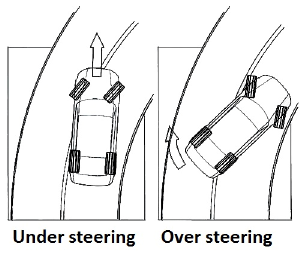
\includegraphics[width=0.7\linewidth]{pictures/Figure-1-Under-steering-vs-over-steering}
	\caption{}
	\label{fig:figure-1-under-steering-vs-over-steering}
\end{figure}

\newpage

\subsection{Throttle by Wire}

After removing the mechanical linkage, a tbw system is usually made up of an pedal and sensors. In paper [9], a hall effect sensor was used, in order to convert the accelerators pedal's position into a proportional analogue voltage, which can be used to control the respective throttle. In full autonomous mode, the sensor is decoupled from the system and the controller mimics the voltage. In order for the driver to have a certain level of feedback, a spring is attached to the pedal, imitating the throttle return spring. 

If each wheel is powered by an individual motor as proposed in [3], there is an electronic control unit (ECU) for every motor, controlling the wheel's rotational speed. While the benefits of a four wheel drive are more known, being able to control all four wheels individually greatly benefits the vehicle's functionality in regards to manoeuvres in critical situations. 
%mentioning "four wheel drive"? benefits such as removing motor, (can crush you [4])

\subsection{Brake by Wire}

A well-implemented bbw system notably increases the vehicle's performance in situation where controlling the vehicle's yaw rate is of importance. A bbw system controls the vehicle yaw rate by differential braking, i.e. when the driver pushes the pedal, the force on each brake is determined by the controller. It can be shown, that a differential braking outperforms steering methods to control the yaw rate.
While a system consisting only of electronic actuators is proposed in \cite{Weidong}, \cite{Aoki} introduces a hydraulic servo brake system with regenerative control for more efficient fuel consumption, coupled with a braking feel that is unaffected by braking control.

%richi schrib du öber das bitte


\section{Vehicle Dynamics, Vehicle Model}

Behind a working dbw system, there needs to be a detailed and complete vehicle model in place. This mathematical model has a determining influence on the controller's performance. When choosing a model, it is important to specify what level of complexity is sufficient. Forces and motions such as wind force, roll, pitch or heave are therefore often neglected. A simpler model may help design a faster controller, while sacrificing precision. It is therefore crucial to identify which states have to be controlled. 

\subsection{Bicycle/single track model}
A simple and common model is the bicycle model, also known as single track model. In papers \cite{Zheng} and \cite{vandersande} this vehicle model has been used. It derives from the double track model, where the left and right wheels have been merged in the front and back axis, creating the single track model. The model accounts for yaw, lateral and longitudinal motion. 

%$
%\dot{x}=
%\begin{bmatrix}
%	\dot{v_{y}} \\ 
%	
%\\	\dot{r_{z}}
%\end{bmatrix} 
%=Ax+B\delta_{rack}
%$
%
%$y=r_{z}=Cx$
%
%$
%A=-
%\begin{bmatrix}
%\dfrac{C_{\alpha1}+C_{\alpha2}}{mv_{x}} &
%\dfrac{C_{\alpha1}a-C_{\alpha2}b}{mv_{x}}+v_{x}\\
%\\
%\dfrac{aC_{\alpha1}-bC_{\alpha2}}{I_{zz} v_{x}} &
%\dfrac{a^2C_{\alpha1}+b^2C_{\alpha2}}{I_{zz}v_{x}}
%\end{bmatrix}
%$
%\\
%
%
%$B=
%\begin{bmatrix}
%\dfrac{C_{\alpha1}}{m}\\
%\\
%\dfrac{aC_{\alpha2}}{I_{zz}}
%\end{bmatrix}
%$
%,
%$C=
%\begin{bmatrix}
%0 & 1
%\end{bmatrix}
%$

By looking at the vehicle dynamics, it becomes apparent that the single track model does not model any non-linearities of the vehicle. Paper \cite{vandersande} accounts for the non-linearity of the tyres by introducing the local gradient of the lateral force. It describes the tyre's cornering stiffness when linearised around a operating point.


\subsection{double-track model}
The double track model is a more complex version of the single track model. 
Paper \cite{Song} uses a combination of the single and double track model. While the double track is implemented to deal with the non-linear characteristic of the vehicle, they argue that a driver usually steers the vehicle according to its linear response. Therefore the bicycle model is introduced as a reference model, so that manoeuvring the vehicle is easy, both in linear and non-linear range.
In paper \cite{Weidong}, the double-track model was used in order to properly adress
brake control design, so that each wheel can be modelled individually.

\subsection{Multi-body modelling}

\cite{vandersande} proposes a multi-body model derived with the software package from MATLAB/Simulink formerly called SimMechanics, now called Simscape Multibody. This can be used to model the car in great detail, as multibody models account for the interconnection of rigid and flexible parts, which make up e.g. a whole car.

\subsection{Tyre modelling}

Tyre modelling is a very complex and heavily research topic in the automotive industry, as tyres are probably the most difficult, but also important components to model. We will therefore not go into too much detail, and keep the concepts and ideas as simple as possible.
The basis of tyre modelling lays in the tyre's elasticity and deformation when subjected to forces. Tyre models are usually divided into models which underlie a physical approach and models which are based on a empirical approach. Empirical models try to recreate the tyre's characteristic curve measured in tests. Physical models are based on the physical properties and forces acting on the tyre in order to create a precise mathematical model. The decision which tyre model to chose often requires to find a balance between computing time and performance.

In the papers, two models stick out. \cite{Se-Wook} makes use of the Pacejka model, also called the magic formula. The name stems the fact that it is a empirical approach and therefore no physical basis was used for this model, but a wide variety of coefficients are in place to tune the existing forces on the tyre, somehow creating a "magic formula".\\
\cite{Weidong} makes use of the Dugoff model. Roughly speaking, the Dugoff model is a analytical model based on the relation between slip angle, tyre stiffness and wheel slip ratio. The exact formulas can be found in paper \cite{Weidong}.

Of course there are many more models to cover, many of which are also adapted and modified versions of previous existing ones. Explaining these and going to much into detail would not beyond the scope of this paper.

\section{Fault tolerance}
The basic requirement for the operation of a dbw system is a fault tolerant system architecture %(Heitzer und Seewald, 2000).

In \cite{Lenkungshandbuch} it is explained, the customers wants his product to be reliable. This of course means that is has to provide a functionality for a designated time under certain circumstances. This leads to the need of balancing between safety and availability. If a product is safe under all circumstances, it may not be available at some times. In the case of failure of a non critical system component, only certain functions of the system are shut down but the overall functionality and availability remains. For example if a wheel rotation sensor fails, only functions that need the current velocity shut down, such as cruise control or the speedometer.

In order to consistently detect faults, sensors should be implemented in groups of three. A faulty sensor can so be overruled by the the two correctly functioning sensors. Control units and actors should be implemented twofold redundant. If an error is detected, the faulty operating unit shuts down and the second control unit or actuator continues with the operation. To lower the cost of redundant implementation, a fault management strategy can be defined. 

In \cite{Lenkungshandbuch} the functionality of a vehicle is separated into the following possible states. 
\begin{enumerate}
	\item faultless
	\item error state 1 (system failure e.g. ABS failure)
	\item error state 2 (function failure)
	\item emergency function (ECU failure of a steering actuator or similar)
	\item function loss (total brake failure	)
\end{enumerate}

For every error state, there is a warning and/or restriction attached. 
\begin{enumerate}
	\item normal operation
	\item warning without restriction, e.g. ABS led lights up
	\item warning with restriction, e.g. maximum velocity limited
	\item "limp home" function enabled, where maximum velocity is drastically limited, to for example provide the possibility to drive to the next service station
	\item shut down or still stand
\end{enumerate}

This is one of the many reasons, why dbw vehicle are usually associated with high costs. Implementing a failsafe system and fallback levels requires a lot more effort, than for standard non-dbw vehicles. Mechanical linkages usually offer enough safety and reliability, which is why less fallback levels exist in non-dbw vehicles. 



\section{Control Algorithms}

\subsection{Control Objective}

Depending on the modelled states, control objectives can vary. The most important however is to stabilise the vehicle's yaw rate around its centre of gravity. Therefore small yaw rate error overshoots are desired. Many controllers also aim to be independent of longitudinal dynamics, as they usually are much slower compared to the rest of the vehicle's dynamics. In order for controllers to perform beyond the capabilities of human drivers, fast error convergence are desired as well. In \cite{vandersande} it is assumed to place the poles such that the bandwidth is higher than around 4 Hz, with the average human reaction time being around 270 ms. 

\subsection{Non-Linearity}

A car's dynamics are non-linear. Especially the tyres non-linear characteristics cause this behaviour. This necessitates a non-linear control algorithm. This can be seen in \cite{vandersande}, where a LQR controller was developed for comparison. From the test results it is apparent that the controller is not able to stabilise the vehicle, resulting in large yaw swaying. This comes down to the fact that high lateral accelerations cause the tyres to behave non-linearly and causing the tyre's parameters to deviate substantially from the fixed parameters of the model.


\subsection{Sliding Mode Control}

Sliding mode is mentioned in papers \cite{Weidong} and \cite{Aoki}. The principle of sliding mode control is that it switches between states in order to slide along a surface which usually corresponds to a linear system. This linear system has the properties of a desired system which is easy to control. The discontinuous signal given to switch between those states can be described as simple input such as "on/off" or "forwards/backwards". These simple control commands make the system insensitive against parameter changes and non-linearities. This of course has the downside of  putting a lot of strain on electric actuators.  	

\subsection{Fuzzy Control}
The basic idea of fuzzy control is to map a set of input variables to a set of output instructions by using a multitude of if then statements. Therefore the inputs are characterized by their membership to a set of fuzzy sets. The degree of membership can be gradual and each input can be a member of multiple fuzzy sets to certain degree. This process of converting a set of crisp input variables to a set of fuzzy membership functions is called fuzzyfication. The next step is to determine the output based the underlying control rules. The membership functions are mapped to a fuzzy output. This fuzzy output is then defuzzyficated to deliver a real world output. In short, each combination of membership of a variable leads output defined by the if then rules.
%(http://www.springer.com/cda/content/document/cda_downloaddocument/9781846284687-c1.pdf.)

This method grants way do deal with a multitude of inputs in a system with unknown environmental parameters. It is especially effective at handling uncertainties and unlinearitites associated with complex control systems such as breaking systems in a car. The nonlinearities can be captured by the control rules.
[1]
\subsection{H-Infinity Control}

\section{Testing, Verification}

Testing can be used to either verify a vehicle model or a controller. Usually the model is tested beforehand, as a faulty model can codetermine a controller's performance. 
In order to study different controllers or vehicle models, it is important to have a fixed set of tests, so that the data is comparable.

In order to verify a model, the real vehicle sensor data needs to be compared to the simulation data of the model. The more they match, the better is the model. To verify the model, the real vehicle undergoes different manoeuvres, such as a slalom and a double lane change at different velocities. This data can then be analysed and used to improve or validate a model. Discrepancies may exist due unmodeled parts or inaccurate parameters.

In order to test a controller's performance a similar test setup is used. Now of course, the real vehicle data needs to be compared to the desired reference manoeuvre.

An especially interesting test setup is the split-$\mu$ braking. In real life, it is a situation which catches most drivers off-guard. This can be the case, when right half of the road is frozen and the other left half not. If the driver now pushes the brakes, it will generate a yaw moment around the vehicle's centre of gravity. This is because, due to the different friction coefficients, the left side generates a significant higher longitudinal force when the brakes are applied. Of course a driver can only react to such a yaw moment via steering and throttle. However the car's controller, able to control each brake individually, is able to counter this moment efficiently.


\section{Results and Discussion}

The goal of this paper was to provide the reader with a basic understanding of the topic drive by wire. While reading into this subject, it became apparent that covering everything in this paper would not be possible, as many concept would require more in-depth knowledge, time and research to explain properly. Because of this, many topics, such as control algorithms or tyre modelling, were merely mentioned to show their importance in the design of a drive by wire system.

\section{Conclusion}

Drive-by-wire system possess the ability to revolutionise the automotive industry. While they provide many technological advantages over standard cars, they still limp behind safety. Due to the increase in complexity and the related high error susceptibility, they have not yet gained the trust of the public, which is obviously a requirement for success. 

\begin{thebibliography}{1}
\bibitem{Weidong}
Weidong Xiang, Paul C. Richardson, Chenming Zhao, Syed Mohammad, 
\emph{Automobile Brake-by-Wire Control System Design and Analysis}, 
NO.1, January 2008.
http://ieeexplore.ieee.org/document/4358463/

\bibitem{Aoki}
Yasushi Aoki, Kenji Suzuki, Hiroshi Nakano, Kohei Akamine, Takaomi Shirase, Kouji Sakai, 
\emph{Development of Hydraulic Servo Brake for Cooperative Control with Regenerative Brake}
http://papers.sae.org/2007-01-0868/

\bibitem{Lenkungshandbuch}
Peter Pfeffer, Manfred Harrer, \emph{Lenkungshandbuch: Lenksysteme, Lenkgefühl, Fahrdynamik von Kraftfahrzeugen} http://www.springer.com/de/book/9783658009762
\textbf{Abschnitt R, Steer-by-wire}

\bibitem{Se-Wook}
Se-Wook Oh, Ho-Chol Chae, Seok-Chan Yun, Chang-Soo Han
\emph{The Design of a Controller for the Steer-by-Wire System}
\url{https://www.jstage.jst.go.jp/article/jsmec/47/3/47_3_896/_article/}

\bibitem{Zheng}
B. Zheng, S. Anwar
\emph{Yaw stability control of a steer-by-wire equipped vehicle via active front wheel steering}
http://www.sciencedirect.com/science/article/pii/S0957415809000804

\bibitem{Yamaguchi}
Yousuke Yamaguchi, Toshiyuki Murakami
\emph{Adaptive Control for Virtual Steering Characteristics on Electric Vehicle Using Steer-by-Wire System}
http://ieeexplore.ieee.org/abstract/document/4689398/

\bibitem{vandersande}
T. van der Sande, P. Zegelaar, I. Besselink, H. Nijmeijer
\emph{A robust control analysis for a steer-by-wire vehicle with uncertainty on the tyre forces}
http://www.tandfonline.com/doi/full/10.1080/00423114.2016.1197407

\bibitem{Song}
Pan Song, Masayoshi Tomizuka, Changfu Zong
\emph{A novel integrated chassis controller for full drive-by-wire vehicles}
http://www.tandfonline.com/doi/abs/10.1080/00423114.2014.991331

\bibitem{SAE Car}
Jordan Kalinowski, Thomas Drage, Thomas Bräunl
\emph{Drive-By-Wire for an Autonomous Formula SAE Car}
http://www.sciencedirect.com/science/article/pii/S1474667016429484



\end{thebibliography}

\end{document}
